% !TEX program = lualatex
\documentclass[11pt,a4paper]{ltjsarticle}

\usepackage[haranoaji]{luatexja-preset}
\usepackage{amsmath,amssymb,mathtools}
\usepackage{booktabs}
\usepackage{graphicx}
\usepackage{geometry}
\geometry{top=25mm,bottom=25mm,left=25mm,right=25mm}
\usepackage{xcolor}
\usepackage{listings}
\usepackage{hyperref}

\lstdefinelanguage{AMPL}{
  morekeywords={set,param,var,minimize,maximize,subject,to,sum,in,within,binary,
    integer,default,card,and,or,not,if,then,else,symbolic},
  sensitive=true,
  morecomment=[l]{\#},
}
\lstset{
  basicstyle=\ttfamily\footnotesize,
  keywordstyle=\color{blue!70!black}\bfseries,
  commentstyle=\color{green!40!black},
  stringstyle=\color{red!60!black},
  frame=single,
  framerule=0.3pt,
  numbers=left,
  numberstyle=\tiny\color{gray},
  breaklines=true,
  columns=fullflexible,
  keepspaces=true,
  showstringspaces=false,
}

\newcommand{\Vset}{V}
\newcommand{\Kset}{K}

\title{複数デポ時間枠付き配送計画問題の混合整数計画による求解と\\
Timefold メタヒューリスティクス解との比較}
\author{Mikio Kubo}
\date{2026年10月7日}

\begin{document}

\maketitle

\begin{abstract}
制約ソルバー Timefold のクイックスタート（vehicle-routing）で扱われている
複数デポ時間枠付き配送計画問題（MDVRPTW）を，2添字アーク定式化に車両割当変数を加えた
混合整数計画として定式化し，AMPL と Python API（amplpy）で実装した．
フィラデルフィア近郊の訪問先 55 件・車両 6 台のインスタンスで，Timefold が出力した解
（総走行時間 82,660 秒）と比較した．
Gurobi は 600 秒の計算で総走行時間 82,210 秒（$-0.54\%$）の解を得た．
同時に得た下界 77,652 秒から，Timefold の解の最適性ギャップは高々 6.1\% であることが分かった．
LP 緩和に部分巡回除去制約を加えると下界は 66,625 秒から 74,453 秒へ改善するが，
時間枠に由来する big-M 制約の弱さのため，最適性の証明には至らなかった．
\end{abstract}

\section{はじめに}

Timefold Solver は，局所探索などのメタヒューリスティクスを用いた制約ソルバーである．
公式のクイックスタート
\footnote{\url{https://github.com/TimefoldAI/timefold-quickstarts/tree/stable/use-cases/vehicle-routing}}
には，車両ごとに異なるデポ（車庫）・容量をもつ時間枠付き配送計画問題の例題が含まれている．
メタヒューリスティクスは短時間で良い解を出すが，その解が最適値からどれだけ離れているかは分からない．

本稿では同じ問題を混合整数計画（MIP）として定式化し，次の 3 点を調べる．
\begin{enumerate}
  \item Timefold の解を MIP ソルバーで改善できるか．
  \item MIP ソルバーの下界から，Timefold の解の品質（最適性ギャップ）をどこまで保証できるか．
  \item 定式化の工夫（アークの前処理，部分巡回除去制約，インジケータ制約）が計算にどう効くか．
\end{enumerate}

\section{問題}

\subsection{Timefold の問題定義}

Timefold のクイックスタートでは，次の制約とスコアで解を評価する．
\begin{itemize}
  \item \textbf{ハード制約}：
    車両容量（\texttt{vehicleCapacity}）と，
    サービス終了時刻が最大終了時刻を超えないこと（\texttt{serviceFinishedAfterMaxEndTime}）．
  \item \textbf{ソフト制約}：
    総走行時間の最小化（\texttt{minimizeTravelTime}）．デポへの帰着も含む．
  \item すべての訪問先を，どれか 1 台の車両に割り当てる．
\end{itemize}
各車両は自分のデポを出発時刻に出発し，訪問先を順に回って同じデポに戻る．
訪問先に最早開始時刻より早く着いた場合は待つ．

\subsection{インスタンス}

Timefold の Web UI から保存した \texttt{フィラデルフィア.json} を用いる．
表\ref{tab:instance} に概要を示す．
このファイルには問題データに加えて Timefold が求めた解（各車両の訪問順）も含まれており，
スコアは \texttt{0hard/0medium/-82660soft}，つまり総走行時間 82,660 秒である．

\begin{table}[htbp]
  \centering
  \caption{インスタンス（フィラデルフィア）の概要}
  \label{tab:instance}
  \begin{tabular}{ll}
    \toprule
    項目 & 値 \\
    \midrule
    訪問先数 & 55（午前枠 28 件，午後枠 27 件） \\
    車両数（＝デポ数） & 6 \\
    車両容量 & 24, 28, 27, 15, 27, 28（合計 149） \\
    総需要 & 81 \\
    出発時刻 & 全車両 7:30 \\
    時間枠 & 午前 8:00--12:00，午後 13:00--18:00 \\
    サービス時間 & 10, 20, 30, 40 分 \\
    \bottomrule
  \end{tabular}
\end{table}

\subsection{走行時間}

Timefold の \texttt{HaversineDrivingTimeCalculator} は，緯度経度から大円距離を求め，
平均時速 50\,km で走行時間に換算する．本稿では次の式を用いた．
\begin{equation}
  d_{pq} = \left\lfloor 2R \arcsin\sqrt{h_{pq}} + 0.5 \right\rfloor \ [\mathrm{m}], \qquad
  t_{pq} = \left\lfloor \frac{3.6\, d_{pq}}{50} + 0.5 \right\rfloor \ [\mathrm{s}],
\end{equation}
ここで $R = 6{,}371{,}000$\,m，
$h_{pq} = \sin^2\frac{\phi_q-\phi_p}{2} + \cos\phi_p\cos\phi_q\sin^2\frac{\lambda_q-\lambda_p}{2}$
（$\phi$ は緯度，$\lambda$ は経度）である．
床関数 $\lfloor x + 0.5 \rfloor$ は Java の \texttt{Math.round} に合わせた四捨五入である．
距離をメートルに丸めてから秒に丸めるこの式は，JSON に記録された 55 区間の走行時間と完全に一致した．
距離を丸めない式や切り捨てを使う式では 1--3 区間で 1 秒ずれる．

\section{定式化}

\subsection{記号}

\begin{itemize}
  \item $\Vset$：訪問先の集合，$\Kset$：車両の集合．車両 $k$ のデポを $o_k$ と書く．
  \item $q_i$：訪問先 $i$ の需要，$s_i$：サービス時間，
        $[e_i, l_i]$：最早開始時刻と最大終了時刻（$l_i$ はサービス\emph{終了}の期限）．
  \item $Q_k$：車両 $k$ の容量，$\tau_k$：出発時刻．
  \item $t_{ij}$：訪問先間，$t_{kj}$：デポ $o_k$ から訪問先 $j$，$t_{ik}$：訪問先 $i$ からデポ $o_k$ への走行時間．
\end{itemize}
時刻は問題の開始時刻（7:30）からの秒で表す．

\subsection{アークの前処理}

時間枠を守れないアークを事前に除く．
\begin{align}
  A &= \{(i,j) \in \Vset\times\Vset : i\neq j,\ e_i + s_i + t_{ij} + s_j \le l_j\}, \\
  S &= \{(k,j) \in \Kset\times\Vset : \tau_k + t_{kj} + s_j \le l_j\}.
\end{align}
たとえば午後枠の訪問先から午前枠の訪問先へのアークは，午後の最早開始時刻 13:00 が
午前の期限 12:00 より遅いので除かれる．
この前処理で訪問先間のアークは 2,970 本から 2,210 本に減る．
デポからのアーク $S$ は 330 本すべて残る．

\subsection{変数}

\begin{itemize}
  \item $x_{ij} \in \{0,1\}$ $((i,j)\in A)$：訪問先 $i$ の次に $j$ を訪問するとき 1．
  \item $y_{kj} \in \{0,1\}$ $((k,j)\in S)$：車両 $k$ の最初の訪問先が $j$ のとき 1．
  \item $z_{ik} \in \{0,1\}$ $(i\in\Vset, k\in\Kset)$：訪問先 $i$ の後に車両 $k$ がデポへ戻るとき 1．
  \item $a_{ik} \in \{0,1\}$ $(i\in\Vset, k\in\Kset)$：訪問先 $i$ を車両 $k$ が担当するとき 1．
  \item $T_i \in [e_i, l_i - s_i]$：訪問先 $i$ のサービス開始時刻．
\end{itemize}

アーク変数 $x$ は車両添字をもたない（2 添字定式化）．
車両ごとにデポ・容量が異なるため，誰がどの訪問先を担当するかを
割当変数 $a$ でルートに沿って伝える．
車両添字付きのアーク $x_{ijk}$ を使う 3 添字定式化に比べ，
2 進変数が約 $|K|$ 分の 1 で済む．

\subsection{モデル}

\begin{align}
  \min\ & \sum_{(i,j)\in A} t_{ij} x_{ij} + \sum_{(k,j)\in S} t_{kj} y_{kj}
          + \sum_{i\in\Vset}\sum_{k\in\Kset} t_{ik} z_{ik} \label{eq:obj}\\
  \text{s.t.}\
  & \sum_{(i,j)\in A} x_{ij} + \sum_{(k,j)\in S} y_{kj} = 1 && j\in\Vset \label{eq:in}\\
  & \sum_{(i,j)\in A} x_{ij} + \sum_{k\in\Kset} z_{ik} = 1 && i\in\Vset \label{eq:out}\\
  & \sum_{(k,j)\in S} y_{kj} \le 1 && k\in\Kset \label{eq:leave}\\
  & \sum_{i\in\Vset} z_{ik} = \sum_{(k,j)\in S} y_{kj} && k\in\Kset \label{eq:return}\\
  & \sum_{k\in\Kset} a_{ik} = 1 && i\in\Vset \label{eq:assign}\\
  & y_{kj} \le a_{jk} && (k,j)\in S \label{eq:startid}\\
  & z_{ik} \le a_{ik} && i\in\Vset,\ k\in\Kset \label{eq:endid}\\
  & x_{ij} + a_{ik} - a_{jk} \le 1 && (i,j)\in A,\ k\in\Kset \label{eq:arcid}\\
  & \sum_{i\in\Vset} q_i a_{ik} \le Q_k && k\in\Kset \label{eq:cap}\\
  & T_j \ge \tau_k + t_{kj} - M_{kj}(1-y_{kj}) && (k,j)\in S \label{eq:tdepot}\\
  & T_j \ge T_i + s_i + t_{ij} - M_{ij}(1-x_{ij}) && (i,j)\in A \label{eq:time}
\end{align}

目的関数 \eqref{eq:obj} は，デポへの帰着を含む総走行時間で，Timefold のソフトスコアと同じである．
制約 \eqref{eq:in}--\eqref{eq:out} は各訪問先の入次数と出次数を 1 にし，すべての訪問先を割り当てる．
制約 \eqref{eq:leave}--\eqref{eq:return} により，各車両はデポを高々 1 回出発し，出発したら同じ数だけデポへ戻る．

制約 \eqref{eq:assign}--\eqref{eq:arcid} は車両の識別を伝える．
$x_{ij}=1$ のとき \eqref{eq:arcid} から $a_{ik} \le a_{jk}$ が全 $k$ について成り立ち，
\eqref{eq:assign} と合わせて $a_{ik} = a_{jk}$ となる．
したがって，デポ $o_k$ を出たルート上の訪問先はすべて $a_{\cdot k}=1$ となり，
\eqref{eq:endid} によりそのルートは自分のデポ $o_k$ に戻る．
これにより，容量制約 \eqref{eq:cap} を車両ごとに書ける．

制約 \eqref{eq:tdepot}--\eqref{eq:time} は時刻の伝播で，到着が早ければ待つことを許す．
最大終了時刻は変数 $T_i$ の上界 $l_i - s_i$ で表す．
サービス時間が正なので，\eqref{eq:time} は訪問先だけからなる閉路も排除する．

\subsection{タイトな big-M}

big-M 係数はアークごとに時間枠から決める．
\begin{equation}
  M_{ij} = l_i + t_{ij} - e_j, \qquad M_{kj} = \tau_k + t_{kj} - e_j.
\end{equation}
$x_{ij}=0$ のとき \eqref{eq:time} の右辺は
$T_i + s_i - l_i + e_j \le e_j$ となる（$T_i + s_i \le l_i$ より）．
これは $T_j$ の下界 $e_j$ 以下なので，制約は効かない．
$M_{kj}$ も同様で，$M_{kj}<0$ の場合も $y_{kj}=0$ のとき右辺は $e_j$ になり妥当である．
一律の大きな定数 $M$ を使うより LP 緩和が強くなる．

\subsection{部分巡回除去制約}

時刻制約 \eqref{eq:time} は整数解の部分巡回を排除するが，LP 緩和では big-M が効かず，
分数値の小さな閉路が多数現れる．
実際，LP 緩和の最適解では 55 件中 41 件の訪問先について，デポから流入するフローが 1 未満だった．
そこで部分巡回除去制約（SEC）
\begin{equation}
  \sum_{(i,j)\in A:\ i,j\in U} x_{ij} \le |U| - 1 \qquad U \subseteq \Vset,\ |U|\ge 2 \label{eq:sec}
\end{equation}
を切除平面として加える．
分離問題は次のように解く．すべてのデポを 1 つの仮想デポ $D$ にまとめ，
LP 解 $(x, y)$ を容量としたネットワークを作る．
各訪問先 $t$ について $D$--$t$ 最小カットを求め，カット値が 1 未満なら
シンク側の集合 $U$ に対する \eqref{eq:sec} が破られている
（入次数制約 \eqref{eq:in} の下で，$U$ への流入が 1 未満であることと \eqref{eq:sec} の違反は同値）．
破られた制約を加えて LP を解き直し，違反がなくなるまで繰り返す．

\section{AMPL による実装}

AMPL の推奨に従い，モデル（\texttt{.mod}）とデータ処理・求解（Python, amplpy）を分けた．
\texttt{.dat} ファイルや \texttt{.run} ファイルは使わない．

\subsection{モデルファイル}

リスト\ref{lst:mod} にモデルファイル \texttt{mdvrptw.mod} の全体を示す．
SEC は添字集合 \texttt{CUTS} と集合族 \texttt{CUT\_SET} で定義し，
Python から集合の中身を更新するだけでカットを追加できる．

\lstinputlisting[language=AMPL,caption={AMPL モデル（\texttt{mdvrptw.mod}）},label=lst:mod]{mdvrptw.mod}

\subsection{インジケータ制約との比較}

AMPL の MP インタフェースでは，時刻制約を
\begin{center}
  \verb|x[i,j] = 1 ==> T[j] >= T[i] + service[i] + t_vv[i,j];|
\end{center}
のようなインジケータ（含意）制約で書ける．big-M を自分で決める必要がなく，読みやすい．
ただし本モデルでは，MP の自動変換によりソルバーに渡るモデルが
3,255 変数から 10,020 変数（うち整数 2,112）に増えた．
Gurobi で 300 秒解いた予備実験（SEC なし，Timefold 解を初期解）では，
暫定解はどちらも 82,210 で，下界はインジケータ版 76,476，タイトな big-M 版 76,210 と大差なかった．
HiGHS ではモデルが大きくなるだけで利点がないため，本稿では線形の big-M 形を採用した．

\subsection{Python（amplpy）}

主要部分を示す．全体は付録に載せる．
リスト\ref{lst:time} は Timefold と同じ走行時間の計算である．

\lstinputlisting[language=Python,firstline=38,lastline=48,firstnumber=38,
  caption={走行時間の計算},label=lst:time]{solve_mdvrptw.py}

リスト\ref{lst:build} はモデルを読み込み，pandas の DataFrame と辞書からデータを渡す部分である．
環境変数 \texttt{AMPL\_PATH} で AMPL 本体の場所を指定できる．
pip で入る \texttt{ampl\_module\_base} はデモライセンス（500 変数まで）なので，
本モデルの求解には正規ライセンスの AMPL が必要である．

\lstinputlisting[language=Python,firstline=101,lastline=120,firstnumber=101,
  caption={モデルの構築とデータの受け渡し},label=lst:build]{solve_mdvrptw.py}

リスト\ref{lst:sec} は SEC の切除平面ループである．
\texttt{relax\_integrality} で LP 緩和を解き，NetworkX の最小カットで違反した SEC を探す．

\lstinputlisting[language=Python,firstline=163,lastline=197,firstnumber=163,
  caption={SEC の分離（切除平面法）},label=lst:sec]{solve_mdvrptw.py}

リスト\ref{lst:solve} は MIP の求解である．
初期解（\texttt{warm}）を変数の初期値として渡し，Gurobi のオプション
\texttt{mip:start=1} で MIP スタートとして使わせる．
AMPL の HiGHS ドライバ（1.11.0）にはこのオプションがない．

\lstinputlisting[language=Python,firstline=200,lastline=227,firstnumber=200,
  caption={MIP の求解},label=lst:solve]{solve_mdvrptw.py}

\section{計算実験}

\subsection{実験環境}

計算機は Intel Xeon W-2140B（3.2\,GHz, 8 コア 16 スレッド），macOS 13 である．
AMPL（20221013 版）から Gurobi 13.0.0 と HiGHS 1.11.0 を呼び，
スレッド数 8，時間上限 600 秒，相対ギャップ 0 を目標に設定した．
すべての MIP には，事前に求めた SEC 32 本を加えた．
比較したのは次の手法である．
\begin{itemize}
  \item \textbf{Timefold}：JSON に保存された解．同じ評価関数で再計算すると，ハード制約違反 0，総走行時間 82,660 秒で一致した．
  \item \textbf{HiGHS}，\textbf{Gurobi}：初期解なし．
  \item \textbf{Gurobi（ウォームスタート）}：Timefold の解を MIP スタートとして与える．
\end{itemize}

モデルの妥当性を確かめるため，まず Timefold の解の変数を固定して AMPL モデルを解いた．
実行可能で，目的関数値は 82,660 と一致した．

\subsection{結果}

表\ref{tab:result} に結果を示す．
ギャップは $(\text{上界}-\text{下界})/\text{上界}$，
「Timefold のギャップ」は $(82{,}660 - \text{下界})/82{,}660$ で，
その下界から保証される Timefold の解の最適性ギャップの上限である．

\begin{table}[htbp]
  \centering
  \caption{計算結果（時間上限 600 秒，単位は秒）}
  \label{tab:result}
  \small
  \begin{tabular}{lrrrrr}
    \toprule
    手法 & 総走行時間 & 下界 & ギャップ & Timefold 比 & Timefold のギャップ \\
    \midrule
    Timefold & 82,660 & -- & -- & -- & -- \\
    LP 緩和 & -- & 66,625 & -- & -- & 19.4\% \\
    LP 緩和 + SEC 32 本 & -- & 74,453 & -- & -- & 9.9\% \\
    HiGHS & 解なし & 75,399 & -- & -- & 8.8\% \\
    Gurobi & 82,257 & 77,004 & 6.4\% & $-0.49\%$ & 6.8\% \\
    Gurobi（ウォームスタート） & \textbf{82,210} & \textbf{77,652} & 5.5\% & $\mathbf{-0.54\%}$ & \textbf{6.1\%} \\
    \bottomrule
  \end{tabular}
\end{table}

SEC の切除平面ループは 5 回の LP 求解（3.7 秒）で収束し，
LP 下界を 66,625 から 74,453 へ 11.7\% 引き上げた．
Gurobi は初期解なしでも Timefold より良い解 82,257 を見つけた．
Timefold の解から始めると，600 秒で 113,710 ノードを探索して 82,210 を得た．
HiGHS は 600 秒で実行可能解を一つも見つけられなかった．

\subsection{ルートの比較}

表\ref{tab:vehicle} に車両ごとの比較を，図\ref{fig:routes} にルートを示す．
Gurobi（ウォームスタート）の解は Timefold の解とほとんど同じで，違いは次の 3 点だけである．
\begin{itemize}
  \item 午前枠の訪問先 32 を車両 2 から車両 4 へ移す．
  \item 午後枠の訪問先 55 を車両 4 から車両 5 へ移す．
  \item 車両 5 の最初の 2 件（訪問先 10 と 39）の順序を入れ替える．
\end{itemize}
車両 1, 3, 6 のルートは変わらない．
車両 2 は 1,216 秒，車両 4 は 37 秒短くなり，車両 5 は 803 秒長くなって，差し引き 450 秒の改善である．
Timefold の局所探索は，2 台の車両の間で訪問先を同時に動かすこの種の改善を見落としていた．

一方，初期解なしの Gurobi の解（82,257）では，車両 4 の訪問先が 5 件に減り，
車両 2 が 7 件を担当するなど，Timefold の解とは異なる割り当てになっていた．
総走行時間がほぼ同じでも構造の違う解が複数あることを示している．

\begin{table}[htbp]
  \centering
  \caption{車両ごとの比較（Timefold / Gurobi ウォームスタート）}
  \label{tab:vehicle}
  \begin{tabular}{crrrrr}
    \toprule
    車両 & 容量 & 訪問数 & 需要 & 走行時間 [s] & 帰着時刻 \\
    \midrule
    1 & 24 & 11 / 11 & 16 / 16 & 15,859 / 15,859 & 18:15 / 18:15 \\
    2 & 28 &  6 / 5  &  9 / 8  & 10,835 / 9,619  & 14:42 / 14:42 \\
    3 & 27 & 14 / 14 & 21 / 21 & 18,016 / 18,016 & 17:21 / 17:21 \\
    4 & 15 &  7 / 7  & 11 / 11 & 11,762 / 11,725 & 15:42 / 14:34 \\
    5 & 27 & 10 / 11 & 15 / 16 & 14,849 / 15,652 & 16:01 / 16:57 \\
    6 & 28 &  7 / 7  &  9 / 9  & 11,339 / 11,339 & 15:13 / 15:13 \\
    \midrule
    計 & 149 & 55 / 55 & 81 / 81 & 82,660 / 82,210 & \\
    \bottomrule
  \end{tabular}
\end{table}

\begin{figure}[htbp]
  \centering
  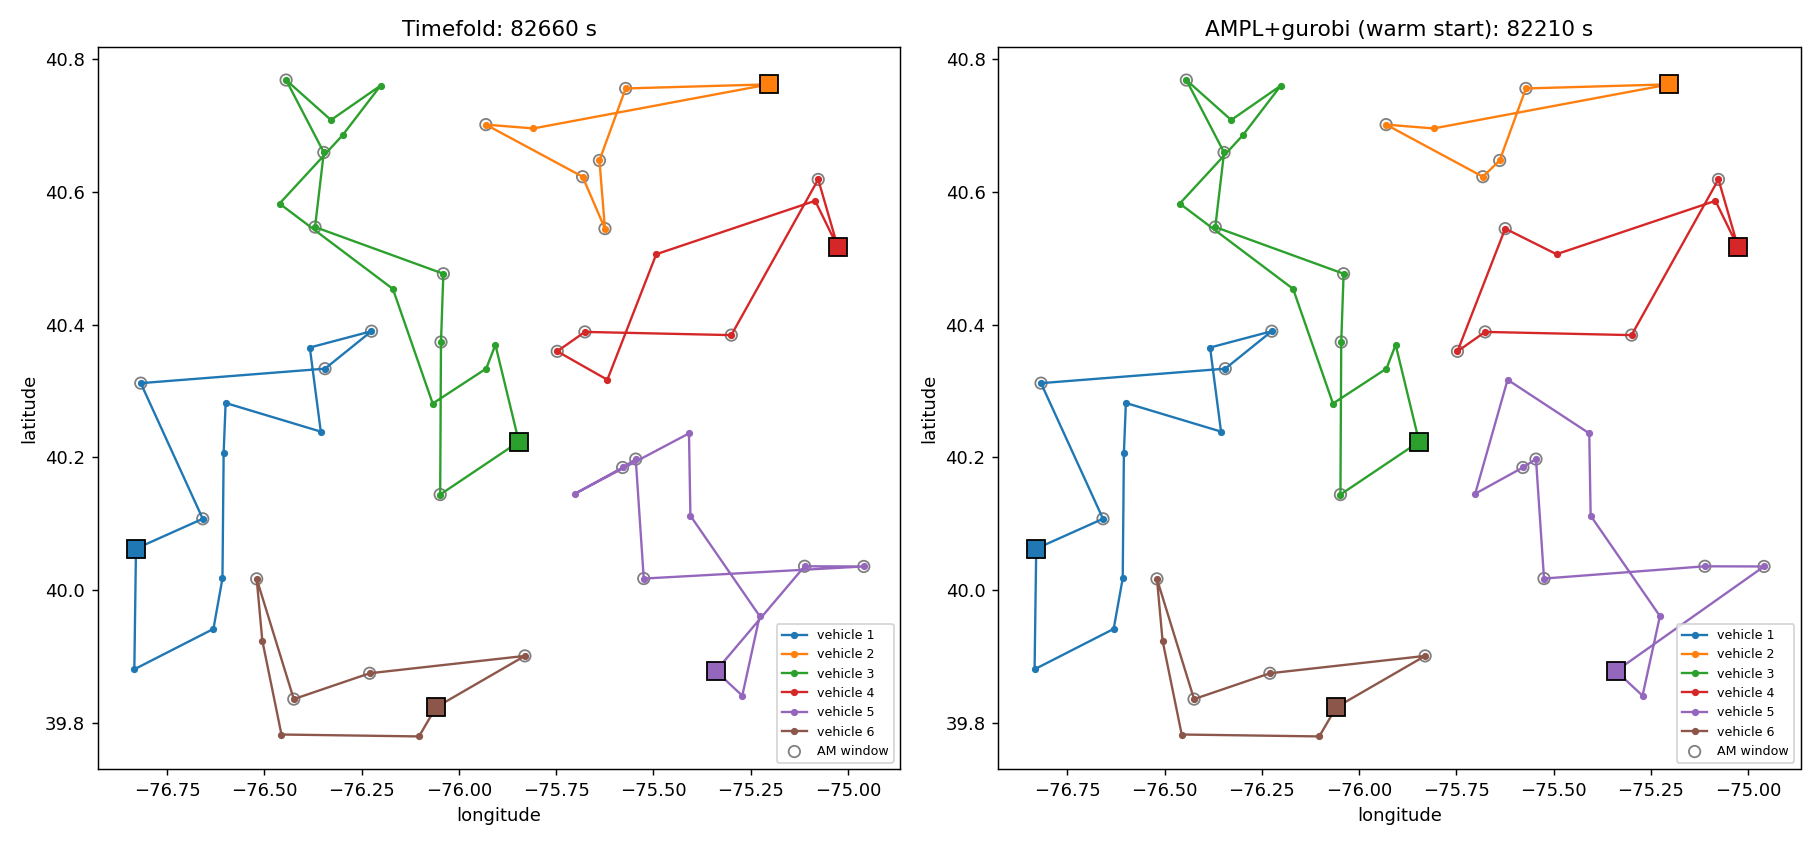
\includegraphics[width=\textwidth]{results/routes_comparison.png}
  \caption{Timefold の解（左）と Gurobi（ウォームスタート）の解（右）．
    四角はデポ，灰色の円は午前枠の訪問先を表す．}
  \label{fig:routes}
\end{figure}

\subsection{考察}

最終的なギャップ 5.5\% の大部分は下界側にあると考えられる．
上界は異なる 3 つの方法（Timefold，Gurobi の初期解なし・あり）で 82,210--82,660 の狭い範囲に収まった．
一方，下界は 600 秒の分枝限定法でも 77,652 までしか上がらなかった．
主な原因は時刻制約 \eqref{eq:time} の big-M だと考えられる．
時間枠の幅（4--5 時間）が 1 区間の走行時間（数十分）に比べて広いので，
$M_{ij}$ をタイトにしても LP 緩和では時刻制約がほとんど効かない．

車両識別の弱さも疑い，車両添字付きアーク $x_{ijk}$ を用いた 3 添字定式化の LP 下界も調べた．
SEC を加えた後の LP 下界は 74,517 で，2 添字版の 74,453 とほとんど変わらなかった．
したがって下界の弱さは，マルチデポの扱いではなく時間枠の扱いに起因する．
最適性を証明するには，時間枠を集合分割（列生成）の価格付け問題で扱う
分枝価格法や，時間枠に関する妥当不等式の追加が有望である．

\section{まとめ}

Timefold の vehicle-routing クイックスタートと同じ複数デポ時間枠付き配送計画問題を
MIP として定式化し，AMPL と amplpy で実装した．
走行時間の計算を Timefold と完全に一致させたので，両者の解を同じ尺度で比較できる．
55 訪問先・6 台のインスタンスでは，Gurobi が Timefold の解を 0.54\% 改善した．
得られた下界から，Timefold の解は最適値から高々 6.1\% 以内であることを保証した．
メタヒューリスティクスの解を MIP の初期解として与えると，
改善と品質保証を同時に行えることが確認できた．

\appendix
\section{Python コード全体}

\lstinputlisting[language=Python,caption={\texttt{solve\_mdvrptw.py}}]{solve_mdvrptw.py}

\end{document}
